% Created by Takeuchi on Feb. 2020
\documentclass[dvipdfmx, 11pt]{beamer}

%%%% Packages %%%%%
%\usepackage{bxdpx-beamer}
%\usepackage{minijs}
%\usepackage{otf}
%\usepackage{tabularx}
%\usepackage{graphicx}
% \usepackage{graphicx}
% \usepackage{amsmath,amssymb,amsthm}
% \usepackage{multirow}
% \usepackage{url}
% \usepackage{tikz}
% \usepackage{alltt}
% \usepackage{bm}
% \usepackage{listings,jlisting}
% \usepackage{listings}
% \lstset{
%  basicstyle=\ttfamily\scriptsize,
%  keepspaces=true,
%  escapechar=|,
%  columns=[l]{fullflexible}
% }

%%%% Fonts %%%%%
\renewcommand{\kanjifamilydefault}{\gtdefault}
% \usepackage{otf} % otfパッケージ
\usepackage[deluxe]{otf} 
\usepackage{txfonts} % 数式・英文ローマン体を Lxfont にする
% \usepackage[T1]{fontenc} % 8bit フォント
% \usepackage{minijs}
% \usepackage{textcomp} % 欧文フォントの追加
% \usepackage[utf8]{inputenc} % 文字コードをUTF-8

%%%%% Beamer %%%%%
\usetheme{Madrid}
\useinnertheme{rectangles}
%\useoutertheme{smoothbars}
\setbeamercolor{enumerate}{fg=white, bg=black}
\usefonttheme{professionalfonts}
\setbeamertemplate{frametitle}[default][center]
\setbeamertemplate{navigation symbols}{}
% \setbeamercovered{transparent} % 好みに応じてどうぞ
\setbeamertemplate{footline}[frame number]
\setbeamercolor{page number in head/foot}{fg=black} % ページ数を表示する
% \setbeamerfont{footline}{size=\normalsize,series=\bfseries}
\setbeamerfont{footline}{size=\scriptsize,series=\mdseries}
\setbeamercolor{footline}{fg=black,bg=black}
\setbeamertemplate{blocks}[rounded][shadow=true]
\setbeamertemplate{items}[ball]
% \setbeamertemplate{enumerate items}[default]
% \setbeamerfont{alerted text}{series=\bfseries}

%%%% My macro %%%%%
%%%%%%%%%%%%%%%%%%%%%%%%%%%%%%%%%%%%%%%%%%%%%%%%%%%%%%%%%%%%%%%%
% User-defined Macro
%%%%%%%%%%%%%%%%%%%%%%%%%%%%%%%%%%%%%%%%%%%%%%%%%%%%%%%%%%%%%%%%
\newcommand{\compress}{\itemsep0pt\parsep0pt\parskip0pt\partopsep0pt}
% \newcommand{\compress}{\itemsep1pt plus1pt\parsep0pt\parskip0pt}
% \newcommand{\code}[1]{\lstinline[basicstyle=\ttfamily]{#1}}
\newcommand{\gringo}{\textit{gringo}}
\newcommand{\clasp}{\textit{clasp}}
\newcommand{\clingo}{\textit{clingo}}
\newcommand{\teaspoon}{\textit{teaspoon}}
\newcommand{\sat}{\textsf{SAT}}
\newcommand{\unsat}{\textsf{UNSAT}}
% \newcommand{\web}[2]{\href{#1}{#2\ \raisebox{-0.15ex}{\beamergotobutton{Web}}}}
% \newcommand{\doi}[2]{\href{#1}{#2\ \raisebox{-0.15ex}{\beamergotobutton{DOI}}}}
% \newcommand{\weblink}[1]{\web{#1}{#1}}
% \newcommand{\imp}{\mathrel{\Rightarrow}}
% \newcommand{\Iff}{\mathrel{\Leftrightarrow}}
% \newcommand{\mybox}[1]{\fbox{\rule[.2cm]{0cm}{0cm}\mbox{${#1}$}}}
% \newcommand{\mycbox}[2]{\tikz[baseline]\node[fill=#1!10,anchor=base,rounded corners=2pt] () {#2};}
% \newcommand{\naf}[1]{\ensuremath{{\sim\!\!{#1}}}}
% \newcommand{\head}[1]{\ensuremath{\mathit{head}(#1)}}
% \newcommand{\body}[1]{\ensuremath{\mathit{body}(#1)}}
% \newcommand{\atom}[1]{\ensuremath{\mathit{atom}(#1)}}
% \newcommand{\poslits}[1]{\ensuremath{{#1}^+}}
% \newcommand{\neglits}[1]{\ensuremath{{#1}^-}}
% \newcommand{\pbody}[1]{\poslits{\body{#1}}}
% \newcommand{\nbody}[1]{\neglits{\body{#1}}}
% \newcommand{\Cn}[1]{\ensuremath{\mathit{Cn}(#1)}}
% \newcommand{\reduct}[2]{\ensuremath{#1^{#2}}}
% \newcommand{\OK}{\mbox{\textcolor{green}{\Pisymbol{pzd}{52}}}}
% \newcommand{\KO}{\mbox{\textcolor{red}{\Pisymbol{pzd}{56}}}}
% \newcommand{\code}[1]{\lstinline[basicstyle=\ttfamily]{#1}}
% \newcommand{\lw}[1]{\smash{\lower2.ex\hbox{#1}}}
\newcommand{\llw}[1]{\smash{\lower3.ex\hbox{#1}}}

\newenvironment{tableC}{%
  \scriptsize
  \renewcommand{\arraystretch}{0.9}
  \tabcolsep = 0.6mm
  % \begin{tabular}[t]{p{6mm}|rlr|rlr|rlr|rlr|rlr}\hline
  %   \multicolumn{1}{l|}{\llw{問題   }} &
  \begin{tabular}[t]{l|rlr|rlr|rlr|rlr|rlr}\hline
    \multicolumn{1}{l|}{\llw{問題}} &
    \multicolumn{3}{c|}{UD1} &
    \multicolumn{3}{c|}{UD2} &
    \multicolumn{3}{c|}{UD3} &
    \multicolumn{3}{c|}{UD4} &
    \multicolumn{3}{c}{UD5} \\
    & 
    \multicolumn{1}{c}{既知の} & & \multicolumn{1}{c|}{ASP} & 
    \multicolumn{1}{c}{既知の} & & \multicolumn{1}{c|}{ASP} & 
    \multicolumn{1}{c}{既知の} & & \multicolumn{1}{c|}{ASP} & 
    \multicolumn{1}{c}{既知の} & & \multicolumn{1}{c|}{ASP} & 
    \multicolumn{1}{c}{既知の} & & \multicolumn{1}{c}{ASP} \\
    & 
    ベスト & &  & 
    ベスト & &  & 
    ベスト & &  & 
    ベスト & &  & 
    ベスト & &  \\
    \hline
  }{%
    \hline
  \end{tabular}
}


%%%%%%%%%%%%%%%%%%%%%%%%%%%%%%%%%%%%%%%%%%%%%%%%%%%%
\title{車両装備仕様問題に対する\\解集合プログラミングの適用}
\author{竹内頼人}
\institute{名古屋大学 工学部 電気電子・情報工学科 情報工学コース 4年}
\date{番原研究室中間発表\\2019年12月20日}
\begin{document}
\begin{frame} {}
 \titlepage
\end{frame}
%%%%%%%%%%%%%%%%%%%%%%%%%%%%%%%%%%%%%%%%%%%%%%%%%%%%
\begin{frame}{車両装備仕様問題}
 \begin{itemize}
 \setlength{\itemsep}{10pt}
  \item \structure{車両装備仕様}とは,自動車のカタログに記載されている自動車のモデル/グレードと装備の組み合わせ
 
  \item \structure{車両装備仕様問題}は,組合せ最適化問題の一種である.

   \item \structure{車両装備仕様問題}は,装備,企業別平均燃費(Corporate Average Fuel Efficiency; CAFE)基準,
      要求仕様に関する制約を満たし,販売台数を最大化する車両装備仕様を求める問題である.
    \begin{itemize}
    \setlength{\itemsep}{7pt}
     \item[-] CAFEとは自動車の燃費規制で,車種別ではなくメーカー全体で出荷台数を加味した平均燃費を算出する方式
      \item[-] アメリカやEUで採用されており,日本でも2020年度燃費基準に採用されることが決定している.
     \end{itemize}
 \end{itemize}
\end{frame}
%%%%%%%%%%%%%%%%%%%%%%%%%%%%%%%%%%%%%%%%%%%%%%%%%%%%
\begin{frame}{解集合プログラミング(Answer Set Programing; ASP)}
 \begin{itemize}
   \setlength{\itemsep}{10pt}
   \item \structure{ASP言語}は,一階論理に基づく知識表現言語の一種である.
   \item \structure{ASPシステム}は,安定モデル意味論[Gelfond and Lifschitz '88]に基づく解集合を計算するシステムである.
   \item 近年,SAT技術を利用した高速なASPシステムが開発され,ロボット工学,システム検証,システム生物学,スケジューリングなど様々な分野への実用的応用が急速に拡大している.
 \end{itemize}
  \begin{exampleblock}{CAFE問題に対してASPを用いる利点}
 	ASP言語の高い表現力により,CAFE問題の各種制約を簡潔に記述できる.
      	系統的探索であるため,解の最適性を保証できる.
      	最適解の列挙が可能である.
 \end{exampleblock}

\end{frame}
%%%%%%%%%%%%%%%%%%%%%%%%%%%%%%%%%%%%%%%%%%%%%%%%%%%%
\begin{frame}{研究目的}
\begin{itemize}
	\setlength{\itemsep}{20pt}
	\item 目的
  	\begin{itemize}
   		\item CAFE問題に対して解集合プログラミングを適用し,その有効性を評価する.
  	\end{itemize}
  	\item 研究内容
  	\begin{enumerate}
		\setlength{\itemsep}{8pt}
   		\item CAFE問題に対する2種類のASP符号化を考案
   		\begin{itemize}
			\item[-] 各種制約を簡潔に記述できることを確認した.
		\end{itemize}
   		\item 企業から提供された実データを用いて,性能評価を行った.
		\begin{itemize}
			\item[-] すべてのデータに対して最適値,あるいは最良値が得られた.
		\end{itemize}
  	\end{enumerate}
\end{itemize}
\end{frame}
%%%%%%%%%%%%%%%%%%%%%%%%%%%%%%%%%%%%%%%%%%%%%%%%%%%%
\begin{frame}{CAFE問題の例}
	3つの仕様を考え,グレードをそれぞれSTD, DX, LXとする.
% 	\begin{center}
% 	\begin{figure}
% 	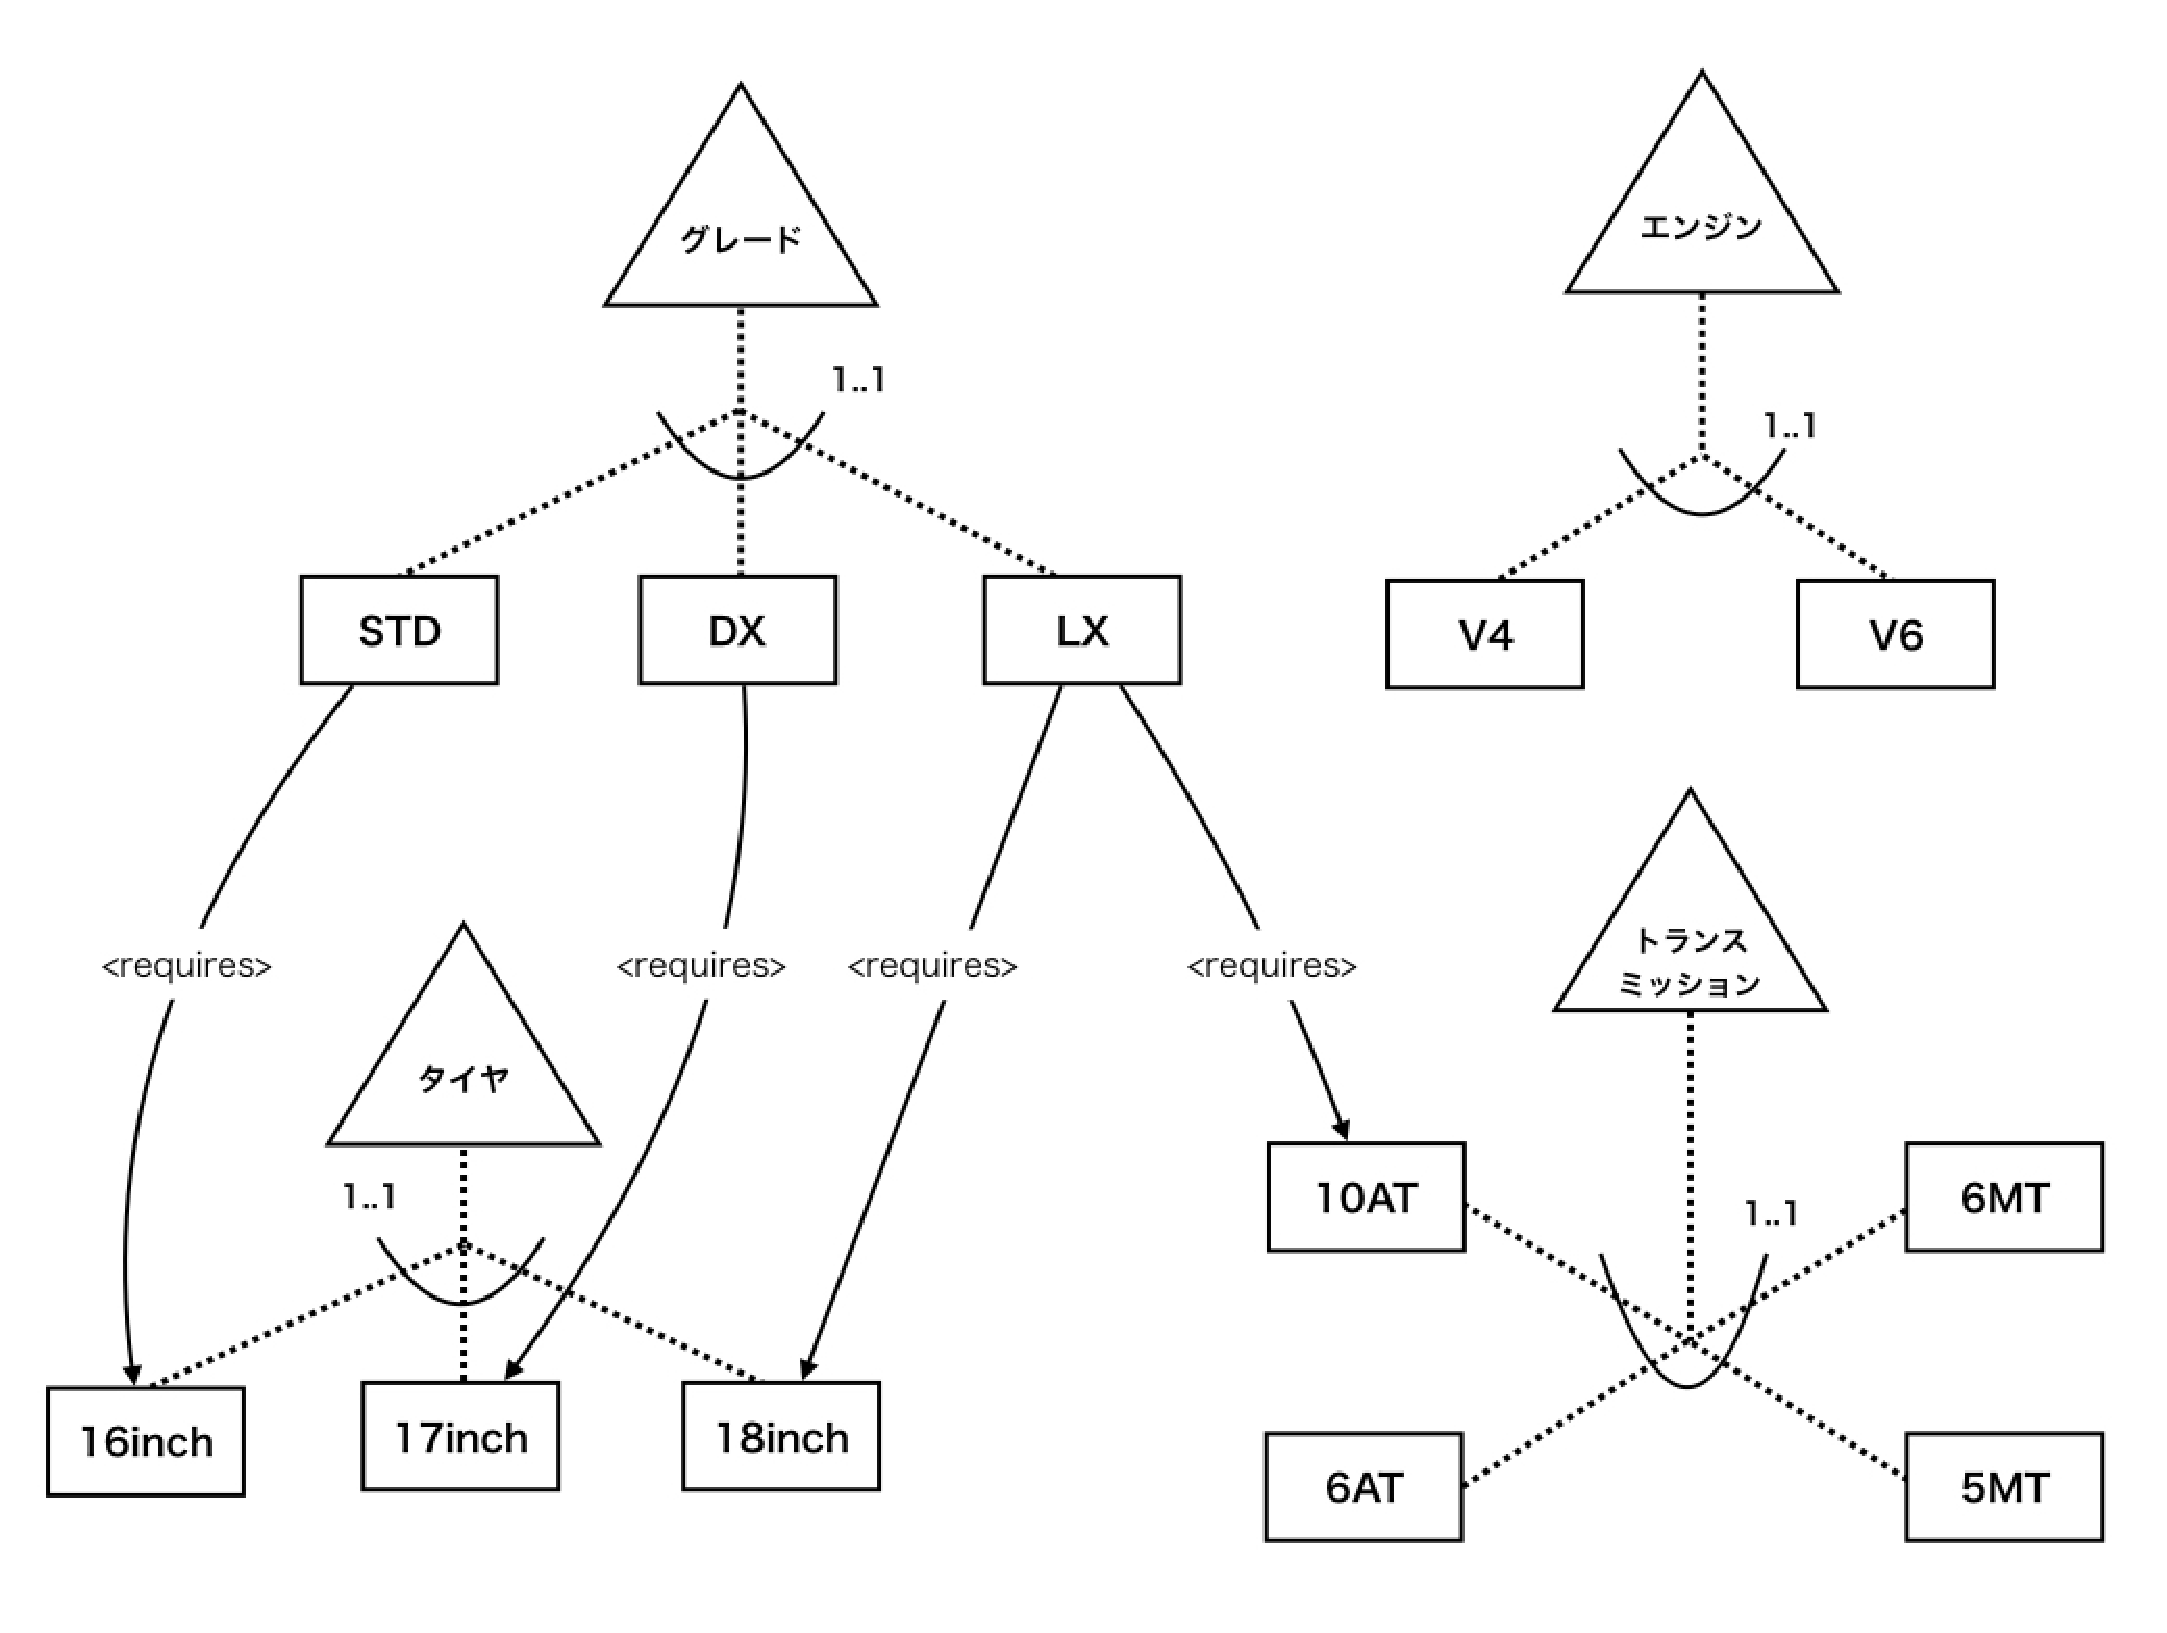
\includegraphics[width=9cm]{pic/OVMmodel001.eps}
% 	\end{figure}
% 	\end{center}
% \end{frame}
% \begin{frame}{CAFE問題の例}
% 	3つの仕様を考え,グレードをそれぞれSTD, DX, LXとする.
% 	\begin{center}
% 	\begin{figure}
% 	\includegraphics[width=9cm]{pic/OVMmodel002.eps}
% 	\end{figure}
% 	\end{center}
\end{frame}
%%%%%%%%%%%%%%%%%%%%%%%%%%%%%%%%%%%%%%%%%%%%%%%%%%%%
\begin{frame}{CAFE制約と販売台数の最大化}
 \begin{itemize}
 \setlength{\itemsep}{20pt}
 \item CAFE制約
 \[ 
 	\underbrace{
		\frac{Fe_{1} \times V_1 + Fe_{2} \times V_2 + Fe_{3} \times V_3 }{V_1 + V_2 + V_3}
	}_{\mbox{平均燃費}}
	\geq 
	\underbrace{X}_{\mbox{CAFE基準値}}
 \]
 \[
Fe_i \mbox{: 仕様iの燃費}\hspace{3em} V_i\mbox{: 仕様iの販売台数}
\]
 \item 販売台数の最大化
 \[
 	max(V_1+V_2+V_3)
 \]
 \end{itemize}
\end{frame}
%%%%%%%%%%%%%%%%%%%%%%%%%%%%%%%%%%%%%%%%%%%%%%%%%%%%
\begin{frame}{最適な車両装備仕様の例}
 	\begin{center}
		\scriptsize
		\begin{tabular}{|l|l|c|c|c|c} \cline{1-5}
			装備分類 & 装備 & \multicolumn{3}{c|}{仕様} & \\ \cline{3-5}
					&		& 1&2&3 & \\ \cline{1-5}
			グレード	& STD & o & & & \\ \cline{2-5}
					& DX & & o & & \\ \cline{2-5}
			 		& LX & & & o & \\ \cline{1-5}
			タイヤ 	& 16 inch & o & & & \\ \cline{2-5}
					& 17 inch & & o & & \\ \cline{2-5}
					& 18 inch & & & o & \\ \cline{1-5}
			トランスミッション	& 5MT  & & o & & \\ \cline{2-5}
							& 6MT & o & & & \\ \cline{2-5}
							& 6AT & & & & \\ \cline{2-5}
							& 10AT & & & o & \\ \cline{1-5}
			エンジン 	& V4 & & & o& \\ \cline{2-5}
					& V6 & o & o & & \\ \cline{1-5}

			\multicolumn{2}{l}{} & \multicolumn{1}{c}{10.4} & \multicolumn{1}{c}{10.2} & \multicolumn{1}{c}{10.1} & 燃費\\ 
			\multicolumn{2}{l}{} & \multicolumn{1}{c}{697} & \multicolumn{1}{c}{750} & \multicolumn{1}{c}{704} & 販売台数\\ 
		\end{tabular}
	\end{center}
	\begin{center}
		平均燃費: 10.2km/L,合計販売台数: 2151台
	\end{center}
\end{frame}
%%%%%%%%%%%%%%%%%%%%%%%%%%%%%%%%%%%%%%%%%%%%%%%%%%%%
\begin{frame}{CAFE問題のASP符号化(提案)}
	\begin{itemize}
	\item CAFE問題に対する2種類の符号化を考案
 		\begin{description}
		\setlength{\itemsep}{10pt}
		\item[符号化1]各制約と目的関数の最大化をそれぞれ符号化
		\item[符号化2]要求仕様制約に関する前処理を追加
		\end{description}
	\vspace{2\baselineskip}
	\item どちらの符号化も10行程度で記述
	\end{itemize}
\end{frame}
%%%%%%%%%%%%%%%%%%%%%%%%%%%%%%%%%%%%%%%%%%%%%%%%%%%%
\begin{frame}{実験概要}
	考案したASP符号化の性能を評価するために比較実験を行なった.
	\begin{itemize}
		\item ASP符号化
		\begin{itemize}
			\item[-] 符号化1,符号化2の2種類
		\end{itemize}
		\item ベンチマーク
		\begin{itemize}
			\item[-] データの大きさの異なるsmall, medium, bigの3種類
		\end{itemize}
		\item ASPシステム
		\begin{itemize}
			\item[-] clingo 5.4.0
		\end{itemize}
		\item システムの設定
		\begin{itemize}
			\item[-] tweety, jumpy の2種類
		\end{itemize}
		\item 制限時間
		\begin{itemize}
			\item[-] 1問あたり30分
		\end{itemize}
	\end{itemize}
\end{frame}
%%%%%%%%%%%%%%%%%%%%%%%%%%%%%%%%%%%%%%%%%%%%%%%%%%%%
\begin{frame}{実験結果: 得られた最良値と最適値}
	\begin{center}
		\scriptsize
		\begin{tabular}{|l|r|r|r|r|r|} \hline
			問題 & CAFE基準値 & 符号化1+t & 符号化2+t & 符号化1+j & 符号化2+j \\ \hline
			small & 8.5 & 6,021* & 6,021* & 6,021* & 6,021* \\
			small & 9.0 & 5,007* & 5,007* & 5,007* & 5,007*   \\
			small & 9.5 & 2,688* & 2,688* & 2,688* & 2,688*       \\
			small & 10.0 & 1,318* & 1,318* & 1,318* & 1,318*       \\
			small & 10.5 & UNSAT & UNSAT & UNSAT & UNSAT       \\ \hline
			medium & 8.5 &  6,010 & 6,021 &  6,002 & 6,021        \\
			medium & 9.0 & 5,595 & 5,595 & 5,595 & 5,496        \\
			medium & 9.5 & 3,447 & 3,447  & 3,447 & 3,447        \\
			medium & 10.0 & 2,245 & 2,205 & 2,243 & 2,245        \\
			medium & 10.5 & 1,170 & 647 & 1,130 & 1,845        \\ \hline
 			big & 8.5 & 5 & UNKNOWN & UNKNOWN & \structure{1,099}        \\
			big & 9.0 & 5 & UNKNOWN  &  \structure{916} & 599         \\
			big & 9.5 & 240 & UNKNOWN &  \structure{550} & 33          \\
			big & 10.0 & 744 & UNKNOWN &  \structure{1,634} & 416         \\
			big & 10.5 & 3 & UNKNOWN  & \structure{538} & 101         \\ \hline
		\end{tabular}
	\end{center}
	\small
	問題small, mediumに対して大きな差は見られない.
	
	問題bigに対して,符号化1+jumpyの組み合わせで最良値が求められることが多かった.
\end{frame}
%%%%%%%%%%%%%%%%%%%%%%%%%%%%%%%%%%%%%%%%%%%%%%%%%%%%
\begin{frame}{実験結果: 制約数の比較}
 	\begin{center}
		\scriptsize
		\begin{tabular}{|l|r|r r r r|} \hline
			問題 & CAFE基準値 & 符号化1+t & 符号化2+t & 符号化1+j & 符号化2+j \\ \hline
			big & 8.5 & 344,416 & 353,557 & \structure{155,645} & 160,121 \\ 
			big & 9.0 & 344,416 & 353,557 & \structure{155,654} & 160,130 \\ 
			big & 9.5 & 344,416 & 353,557 & \structure{155,672} & 160,146 \\ 
			big & 10.0 & 344,416 & 353,557 & \structure{155,681} & 160,155 \\ 
			big & 10.5 & 344,416 & 353,557 & \structure{155,690} & 161,009 \\ \hline
		\end{tabular}
	\end{center}
	制約の数はjumpyはtweetyの半分ほどで,符号化1+jumpyの組み合わせが最も少ない.
	
	この制約の数の差が問題bigにおける目的関数の値につながっていると考えられる.

\end{frame}
%%%%%%%%%%%%%%%%%%%%%%%%%%%%%%%%%%%%%%%%%%%%%%%%%%%%
\begin{frame}{まとめ}
	CAFE問題に対してASPを適用し,その有効性を評価するために以下を行なった.
	\begin{itemize}
	\item CAFE問題に対する2種類のASP符号化を考案した.
		\begin{itemize}
		\item[-] 各種制約を合計10行程度で簡潔に記述することができた.
		\end{itemize}
	\item 企業から提供された実データに対して性能評価を行なった.
		\begin{itemize}
		\item[-] すべてのデータに対して最適値,あるいは最良値が見つかった.
		\item[-] 符号化とオプションの組み合わせによって制約数が大きく変わり,より大きい目的関数の値が求まった.
		\end{itemize}
	\end{itemize}
	\begin{alertblock}{今後の課題}
		\begin{itemize}
		\item 大きいデータでも最適値を求めるためのASP符号化の考案
		\item 最適値が求まった場合の複数解の列挙
		\end{itemize}
	\end{alertblock}
\end{frame}
%%%%%%%%%%%%%%%%%%%%%%%%%%%%%%%%%%%%%%%%%%%%%%%%%%%%
\begin{frame}{各ベンチマークの詳細}
	\begin{center}
		\begin{tabular}{ l|r r r }
		問題		& 装備分類数	& 装備数		& 要求制約数 	\\ \hline
		small	& 8			& 21		& 12		\\
		medium	& 86		& 226		& 163		\\
		big		& 315		& 1337		& 172		\\
		\end{tabular}
	\end{center}
	\begin{center}
		mediumは現実的なサイズの問題
	\end{center}
\end{frame}
\end{document}
